\documentclass{article}

\usepackage[final]{neurips_2019}

\usepackage[utf8]{inputenc}
\usepackage[T1]{fontenc}
\usepackage{hyperref}
\usepackage{url}
\usepackage{booktabs}
\usepackage{amsfonts}
\usepackage{amsmath}
\usepackage{nicefrac}
\usepackage{microtype}
\usepackage{graphicx}
\usepackage{xcolor}

\title{
  Where Reasoning Branches: \\
  How Preference Pair Construction Shapes DPO \\
  for Mathematical Reasoning \\
  \vspace{1em}
  \small{\normalfont Stanford CS224N Custom Project}
}

\author{
  Duy Nguyen \\
  Department of Computer Science \\
  Stanford University \\
  \texttt{duynguy@stanford.edu}
}

\begin{document}

\maketitle

\begin{abstract}
We originally wanted to test whether a co-evolving strategy scaffold could leave a lasting imprint on model weights during RL training for math reasoning.
It did not---at 7B--8B scale the model learned to lean on the scaffold's structure instead of internalizing its content, and our attempts to detect reasoning-critical branch points through token entropy and hidden-state probes also came up short.
What we were left with was the data infrastructure we had built: rollouts, error-position identification, and correction generation.
We used it to compare two ways of constructing DPO preference pairs on Qwen3-8B over MATH-500.
Natural rollout pairs (correct vs.\ incorrect solutions to the same problem) consistently helped; correction pairs (self-repair continuations at identified error positions) consistently hurt.
A matched replication on the correction side brought the total to 11 conditions; 10 of 11 went the way we expected.
When we ablated what in the correction data was actually causing the drop, it turned out to be the failed-reasoning prefix, not the ``wait, let me reconsider'' rhetoric we initially suspected.
\end{abstract}

\section{Key Information}
\begin{itemize}
    \item Mentor: Mirac Suzgun
    \item External collaborators: None
    \item Sharing project: No
\end{itemize}

%--------------------------------------------------
\section{Introduction}
\label{sec:intro}
%--------------------------------------------------

This project started from Dynamic Cheatsheet~\cite{suzgun2025dc}, which maintains a persistent strategy scaffold in context during inference.
We asked whether co-evolving such a scaffold with RL weight updates could produce durable weight absorption---strategies that persist after the scaffold is removed.
A kill-test at 3B and 7B scale (Appendix~\ref{app:trajectory}) showed the opposite: at this scale the model learned to condition on the scaffold's structure rather than absorb its content into weights.
We then tried to identify where reasoning branches---positions where the model's next token choice determines whether it reaches the right answer---using token entropy and hidden-state probes, but neither produced a reliable signal (42\% false-positive rate on token entropy; hidden-state probes could not beat a position-only baseline).

The scaffold and probe work did not pan out, but the infrastructure we built for it---rollouts, error-position identification via DEEP-GRPO~\cite{deepgrpo2026}, and correction generation---turned out to be useful for a different question.
We ended up comparing two ways of constructing preference pairs for DPO~\cite{rafailov2023dpo}, and that comparison is what this paper reports.
Lai et al.~\cite{lai2024stepdpo} applied DPO to math reasoning by having GPT-4o identify the first wrong step and generate a correction.
Kumar et al.~\cite{kumar2024score} showed that SFT on self-corrections fails from distributional mismatch, but since DPO learns relative preferences rather than imitating targets, it was not obvious the same problem would apply.

We built preference pairs two ways on MATH-500 with Qwen3-8B.
Correction-based pairs truncate an incorrect rollout at an identified error position and generate a self-repair continuation; all 3 correction conditions hurt performance ($-0.8$ to $-3.8$pp).
Rollout-based pairs take a naturally sampled correct solution and an incorrect one to the same problem, with no correction generation or external judge; all 5 rollout conditions help ($+0.6$ to $+3.2$pp).
We ran a matched-hyperparameter replication on the correction side, bringing the total to 11 conditions.
Ten of 11 move in the predicted direction (sign test $p = 0.012$; Demsar~\cite{demsar2006}).
Individual comparisons are underpowered and the two experiments use different baselines, so we discuss these caveats in \S\ref{sec:results}.
An ablation (\S\ref{sec:analysis}) traces the correction failure to the failed-reasoning prefix that precedes each correction: stripping the self-repair rhetoric alone does not help, but removing the failed prefix recovers performance to baseline.

%--------------------------------------------------
\section{Related Work}
\label{sec:related}
%--------------------------------------------------

Three bodies of prior work are relevant: preference data construction, error-position identification in reasoning, and the failure modes of self-correction training.

On the data side, Khaki et al.~\cite{datasalgorithm2025} make the provocative claim that the dataset \emph{is} the algorithm---that DPO outcomes depend more on how pairs are constructed than on optimizer details.
Ivison et al.~\cite{unpackingdpo2024} and Liu et al.~\cite{whatmatters2025} provide supporting evidence from different angles: sampling strategy and chosen-response quality, respectively.
Our experiments were not designed to test this, but the correction-vs-rollout split is a concrete case where data construction flips the outcome sign.

For error-position identification, we build on Step-DPO~\cite{lai2024stepdpo}, which uses GPT-4o to find the first wrong step and generate a correction.
The step-level verification idea goes back to Lightman et al.~\cite{lightman2023verify}; Math-Shepherd~\cite{mathshepherd2024} and OmegaPRM~\cite{omegaprm2024} automated it at scale.
We use DEEP-GRPO's~\cite{deepgrpo2026} depth-biased selection instead of an external judge, which is cheaper but limits us to problems where the model already produces both correct and incorrect rollouts.
GRPO~\cite{shao2024grpo} provides the underlying rollout infrastructure.
We do not compare against Step-DPO directly (different scale, model, and task split).

Our negative results on correction pairs connect to the self-correction failure literature.
Kumar et al.~\cite{kumar2024score} showed that SFT on model-generated corrections fails from distributional mismatch, and Huang et al.~\cite{huang2024selfcorrect} found that correction prompts bias models toward changing answers even when the original was right.
We expected DPO's contrastive objective to be less susceptible, since it does not directly imitate the chosen text.
It was not---correction pairs degraded performance in all 3 of our conditions, and our ablation (\S\ref{sec:analysis}) traces the problem to the failed-reasoning prefix rather than the correction rhetoric itself.

%--------------------------------------------------
\section{Approach}
\label{sec:approach}
%--------------------------------------------------

\subsection{Rollout Generation and Filtering}

We evaluate Qwen3-8B~\cite{qwen3_2026} on MATH-500~\cite{hendrycks2021math}.
For each of the 500 problems, we generate $N = 8$ rollouts using vLLM with temperature $T = 0.7$.
We retain problems where at least one rollout is correct and at least one is incorrect ($1 \leq n_{\text{correct}} < N$), since constructing preference pairs requires both outcomes.
This yields 141 problems (28.2\%); the remaining 311 (62.2\%) are solved by all rollouts and 48 (9.6\%) by none.

\subsection{Preference Pair Construction}

We construct preference pairs from the mixed-outcome set using two data sources (Figure~\ref{fig:pipeline}).

\paragraph{Correction-based pairs.}
We identify error positions using DEEP-GRPO's~\cite{deepgrpo2026} depth-biased selection:
\begin{equation}
    Q(t) = P_\phi(\text{success} \mid r_t) \cdot \left(\frac{t}{T}\right)^\gamma, \quad \gamma = 2
\end{equation}
where $P_\phi = \sigma(w \cdot r_t + b)$ is a logistic regression on normalized depth $r_t = t/T$, fit online with bootstrap initialization on the first 10 problems.
Segmentation uses paragraph boundaries (\texttt{\textbackslash n\textbackslash n}) rather than fixed token chunks.
At each error position, we truncate the incorrect rollout and prompt the model to generate a correction starting with ``Wait, let me reconsider\ldots''
The chosen response is the corrected text; the rejected is the original erroneous continuation.
This produces 189 pairs per condition across three pair-selection strategies: random subset, late divergence ($>10\%$ depth), and early divergence ($\leq 10\%$ depth).

\paragraph{Rollout-based pairs.}
For each mixed-outcome problem, we pair a naturally sampled correct rollout with a naturally sampled incorrect one.
No correction generation, no external judge---both chosen and rejected responses come from the model's own generation distribution.
This produces 150--228 pairs depending on filtering.
We test two structuring variants: \textbf{full-trajectory} (problem as prompt, entire solutions as chosen/rejected) and \textbf{prefix-split} (extend the prompt with the shared prefix up to the divergence position identified during rollout comparison, snapped to paragraph boundaries, and use only the post-divergence suffixes).
The prefix-split variant is motivated by an observation about DPO's gradient (\S\ref{sec:analysis}).

\begin{figure}[t]
    \centering
    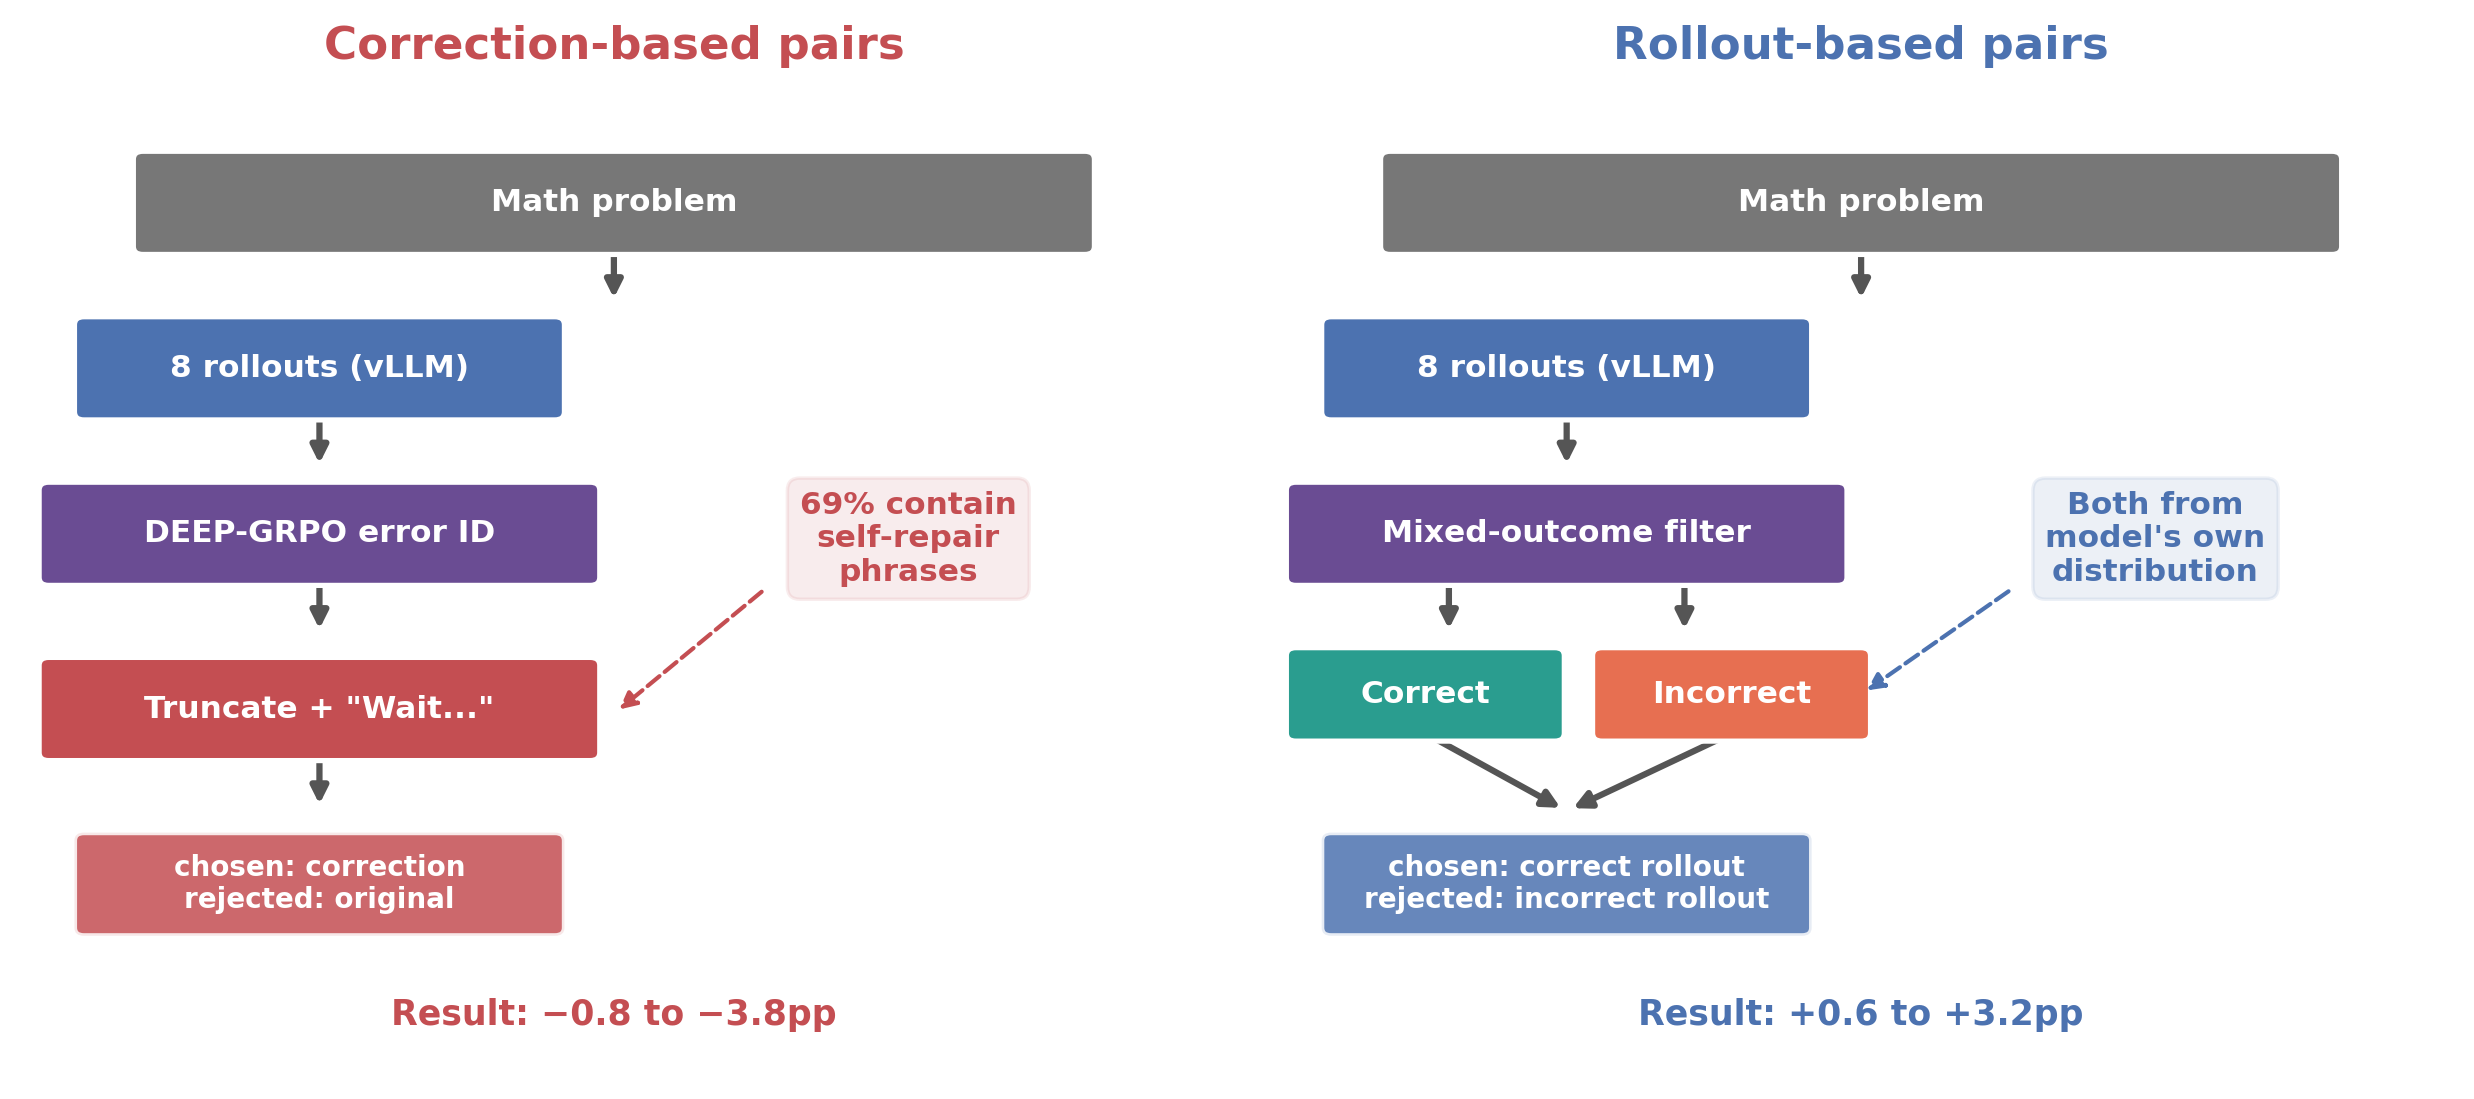
\includegraphics[width=\linewidth]{figures/pipeline_diagram.png}
    \caption{The two data-construction pipelines. Correction-based pairs inject out-of-distribution ``Wait\ldots'' text; rollout-based pairs use only the model's own generations.}
    \label{fig:pipeline}
\end{figure}

%--------------------------------------------------
\section{Experiments}
\label{sec:experiments}
%--------------------------------------------------

\subsection{Data}

We use MATH-500~\cite{hendrycks2021math}, which contains 500 problems spanning 5 difficulty levels and 7 subjects.
After mixed-outcome filtering ($1 \leq n_{\text{correct}} \leq 7$ out of 8 rollouts), 141 problems (28.2\%) yield usable preference pairs, with a mean accuracy of 72.9\% across all rollouts.

\subsection{Evaluation Method}

We evaluate greedy pass@1 ($T = 0$) on all 500 problems.
Each condition is compared against its base model using McNemar's test~\cite{demsar2006}, which counts problems where exactly one model is correct and tests whether those disagreements are one-sided.
Within each experiment we apply Benjamini-Hochberg correction.
Because individual comparisons are underpowered at this scale, we also report the sign test~\cite{demsar2006} over the full set of conditions to check directional consistency.

\subsection{Experimental Details}

All experiments use Qwen3-8B with QLoRA~\cite{dettmers2023qlora} ($r = 64$, $\alpha = 128$).
The two experiments use different training pipelines:
\begin{itemize}
    \item \textbf{Correction DPO}: starts from an SFT checkpoint (Qwen3-8B fine-tuned on 465 clean traces, 77.4\% pass@1), $\beta = 0.2$, learning rate $5 \times 10^{-6}$, 3 epochs, 189 pairs per condition.
    \item \textbf{Rollout DPO}: starts from the same SFT checkpoint architecture but a separate merge yielding 74.2\% pass@1, $\beta = 0.1$, learning rate $2 \times 10^{-5}$, 1--3 epochs, 150--228 pairs per condition.
\end{itemize}
Because the baselines (77.4\% vs 74.2\%), hyperparameters, and epoch counts differ, we cannot directly compare effect sizes across the two experiments.
We use the sign test (\S\ref{sec:results}) for directional consistency and discuss the need for a matched replication in \S\ref{sec:conclusion}.

\subsection{Results}
\label{sec:results}

\paragraph{Rollout-based DPO.}

Table~\ref{tab:rollout} shows the rollout conditions.
Every condition outperforms the SFT base (74.2\%), ranging from $+0.6$ to $+3.2$pp.
Two reach raw $p < 0.05$ by McNemar's test, but neither survives Benjamini-Hochberg correction (adjusted $p = 0.107$)---not surprising with only 150--228 training pairs.

\begin{table}[t]
    \centering
    \caption{Rollout-based DPO results. Base: SFT checkpoint (74.2\%). All use $\beta = 0.1$. $^*$Raw $p < 0.05$ (adjusted $p = 0.107$).}
    \vspace{0.5em}
    \begin{tabular}{llcccc}
        \toprule
        Model & Type & Pairs & Pass@1 & $\Delta$ & Raw $p$ \\
        \midrule
        SFT base & --- & --- & 74.2\% (371/500) & --- & --- \\
        Rollout 1 & prefix-split & 228 & 74.8\% (374/500) & $+0.6$pp & $0.761$ \\
        Rollout 2 & full-traj, 1ep & 150 & 75.2\% (376/500) & $+1.0$pp & $0.511$ \\
        Rollout 3 & full-traj, 3ep & 150 & 75.6\% (378/500) & $+1.4$pp & $0.349$ \\
        Rollout 4 & prefix-split & 150 & 76.6\% (383/500) & $+2.4$pp & $0.036^*$ \\
        Rollout 5 & full-traj, 1ep & 228 & 77.4\% (387/500) & $+3.2$pp & $0.026^*$ \\
        \bottomrule
    \end{tabular}
    \label{tab:rollout}
\end{table}

\paragraph{Correction-based DPO.}

All three correction conditions (Table~\ref{tab:correction}) scored below the SFT base (77.4\%).
Random pair selection does worst ($-3.8$pp, $p = 0.016$), while early-divergence loses only $-0.8$pp ($p = 0.678$).
The gap between the two is significant ($+3.0$pp, $p = 0.036$), likely because earlier error positions preserve more correct reasoning before the self-repair text begins.

\begin{table}[t]
    \centering
    \caption{Correction-based DPO results. Base: SFT checkpoint (77.4\%). $\beta = 0.2$, 3 epochs, 189 pairs. $^*p < 0.05$.}
    \vspace{0.5em}
    \begin{tabular}{llccc}
        \toprule
        Model & Pair Selection & Pass@1 & $\Delta$ & $p$ \\
        \midrule
        SFT base & --- & 77.4\% (387/500) & --- & --- \\
        Correction 1 & Random subset & 73.6\% (368/500) & $-3.8$pp & $0.016^*$ \\
        Correction 2 & Late div.\ ($>$10\%) & 75.0\% (375/500) & $-2.4$pp & $0.119$ \\
        Correction 3 & Early div.\ ($\leq$10\%) & 76.6\% (383/500) & $-0.8$pp & $0.678$ \\
        \bottomrule
    \end{tabular}
    \label{tab:correction}
    \vspace{0.3em}
    {\small Correction 3 vs Correction 1: $+3.0$pp, $p = 0.036^*$.}
\end{table}

\paragraph{Directional consistency.}

With 500 evaluation problems and effect sizes of 1--3pp, individual McNemar tests are underpowered, so we also report directional consistency.
Before the matched replication, all 3 correction conditions fell below their base and all 5 rollout conditions exceeded theirs (8/8, $p = 0.008$ by sign test; Demsar~\cite{demsar2006}).
After adding 3 replication conditions, one of which crosses slightly above base, the count is 10/11 ($p = 0.012$).

We note two caveats on the sign test.
First, the two experiments use different SFT checkpoints (77.4\% vs 74.2\%), different $\beta$, learning rate, and epoch counts, so the 11 conditions are not drawn from the same experimental setup.
Second, conditions within each experiment share the same evaluation set, inflating their non-independence.

\paragraph{Matched replication.}
To partially address the confound, we re-ran the 3 correction conditions with matched hyperparameters ($\beta = 0.1$, lr $= 2 \times 10^{-5}$, 1 epoch) starting from a fresh SFT checkpoint (76.8\%).
Random dropped $-1.0$pp ($p = 0.560$), late-divergence $-2.2$pp ($p = 0.144$), and early-divergence rose $+0.6$pp ($p = 0.771$).
Two of three conditions went negative; the early-divergence exception ($+0.6$pp, $p = 0.771$) is well within noise.
Including the replication, the overall directional count is 10/11 ($p = 0.012$ by sign test).

\begin{figure}[t]
    \centering
    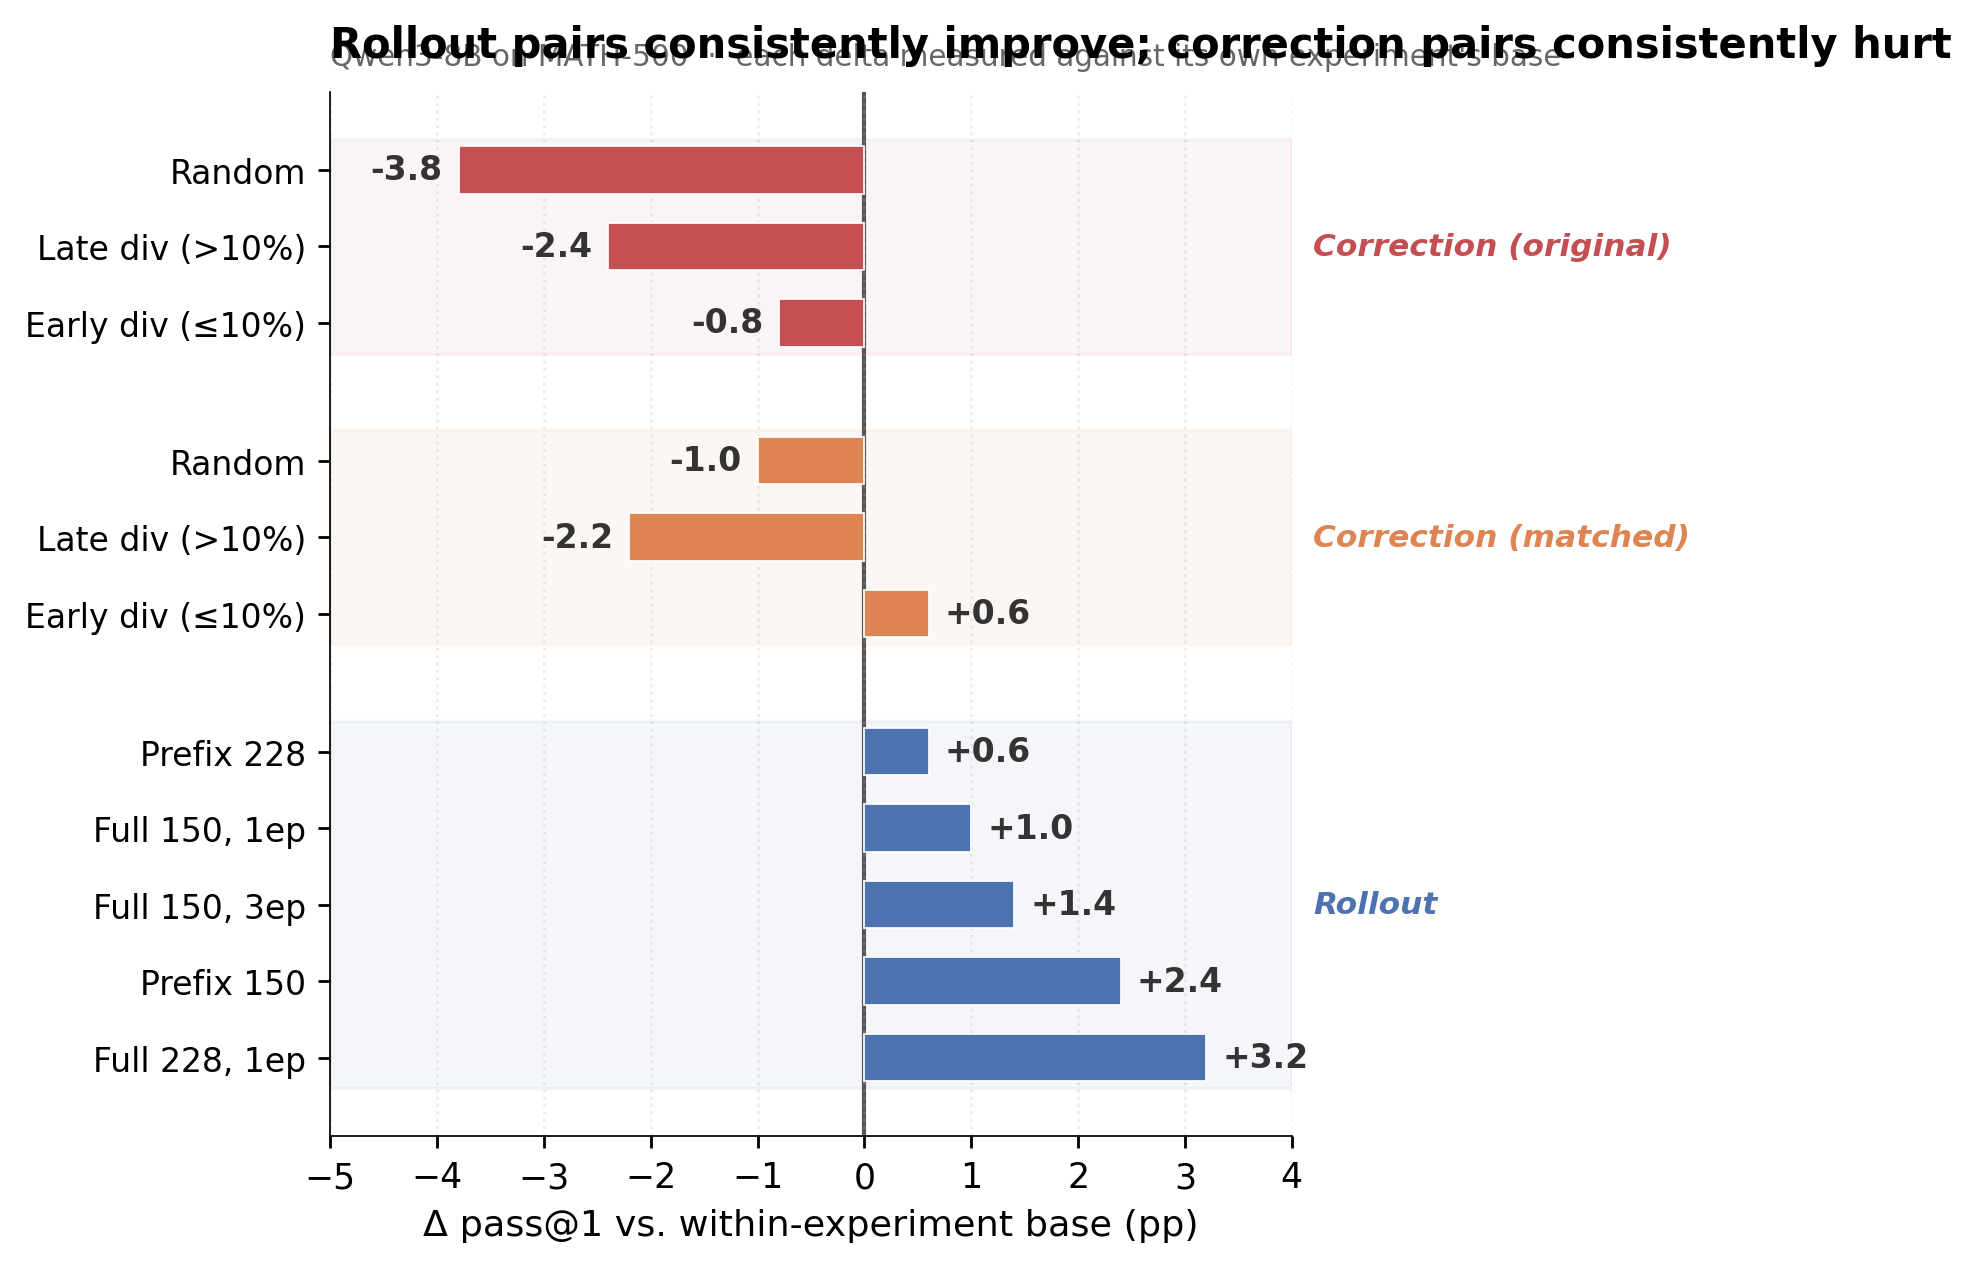
\includegraphics[width=\linewidth]{figures/main_results.png}
    \caption{Pass@1 across all conditions. Left: correction-based (most below base). Right: rollout-based (all above base). Dashed lines show respective base models.}
    \label{fig:all_conditions}
\end{figure}

\paragraph{Null result: Full-trajectory $\approx$ prefix-split.}
With 150 pairs, prefix-split leads by $+1.4$pp ($p = 0.311$); with 228 pairs, full-trajectory leads by $+2.6$pp ($p = 0.066$).
Neither difference is significant, and the direction reverses between the two pair counts.
Section~\ref{sec:analysis} discusses why the two approaches produce similar results.

%--------------------------------------------------
\section{Analysis}
\label{sec:analysis}
%--------------------------------------------------

\paragraph{Distributional mismatch in corrections.}
Our correction pipeline prepends a fixed transition phrase (``Wait, let me reconsider this step\ldots'') before generating continuations.
In the correction data, roughly 69\% of generated corrections contain self-repair rhetoric (``actually,'' ``wait,'' ``let me re-evaluate'').
Less than 1\% of the model's natural generations contain this kind of language.
When DPO trains on correction pairs, it learns to prefer responses with self-repair markers, and we observed verbose hedging at inference even on problems where the original reasoning was correct.
Kumar et al.~\cite{kumar2024score} documented the same distributional mismatch for SFT; we see it here in DPO as well.

\paragraph{Ablation: rhetoric vs.\ prefix.}
To pin down what in the correction data actually causes the drop, we ran two ablations on the late-divergence condition (Table~\ref{tab:ablation}).
First, we neutralized the self-repair rhetoric by replacing ``Wait, let me reconsider\ldots'' with a neutral continuation marker, keeping the failed prefix intact.
This did not help: pass@1 dropped $-2.0$pp ($p = 0.21$), nearly identical to the unmodified correction ($-2.2$pp in the original experiment).
Second, we removed the failed prefix entirely, presenting only the post-divergence correction as the chosen response.
This recovered performance to within $-0.2$pp of base ($p = 1.0$, discordant pairs 23 vs 24).

So the self-repair rhetoric (``wait,'' ``actually'') does not seem to be what causes the drop---the failed reasoning that precedes the correction is the more likely culprit.
When DPO sees a chosen response that begins with incorrect reasoning followed by a course correction, it learns to associate that incorrect context with the preferred signal.
Stripping the prefix removes this confound and the correction data stops hurting.

\begin{table}[t]
    \centering
    \caption{Ablation on late-divergence correction pairs. Base: 76.0\% (380/500). All use $\beta = 0.1$, 1 epoch.}
    \vspace{0.5em}
    \begin{tabular}{lccc}
        \toprule
        Variant & Pass@1 & $\Delta$ & McNemar $p$ \\
        \midrule
        Base (SFT checkpoint) & 76.0\% (380/500) & --- & --- \\
        Neutralized rhetoric & 74.0\% (370/500) & $-2.0$pp & 0.212 \\
        Neutralized + no prefix & 75.8\% (379/500) & $-0.2$pp & 1.000 \\
        \bottomrule
    \end{tabular}
    \label{tab:ablation}
\end{table}

\paragraph{Distributional alignment in rollouts.}
In rollout pairs, both sides come from the same sampling process (same temperature, same model, no injected text).
Both the chosen and rejected responses come from the same sampling process, so neither contains injected text or external edits.
The chosen response happens to be correct, but stylistically it is indistinguishable from the model's normal output.
Liu et al.~\cite{whatmatters2025} argue that chosen-response quality is what drives DPO gains; rollout pairs satisfy that without the distributional artifacts we see in corrections.

\paragraph{Shared-prefix cancellation.}
In the rollout-based setup, the chosen and rejected responses share an identical prefix up to the divergence point (Figure~\ref{fig:gradient}).
DPO's gradient is $\nabla \log \pi(y_w) - \nabla \log \pi(y_l)$; shared-prefix tokens contribute the same value to both terms and cancel.
SFT has no such cancellation---it reinforces all tokens including the shared prefix.
In our data, Qwen3-8B traces average $\sim$800 tokens and divergence is often past 90\% depth, so the prefix-to-suffix ratio is around 8--10$\times$.
Under SFT, most of the gradient comes from that long shared prefix rather than the short suffix where the answers actually differ.

If this cancellation is real, manually stripping the shared prefix (prefix-split DPO) should not help much over full-trajectory DPO.
In our experiments (\S\ref{sec:results}), the two are statistically indistinguishable, which is consistent with the argument though not proof of it.

\begin{figure}[t]
    \centering
    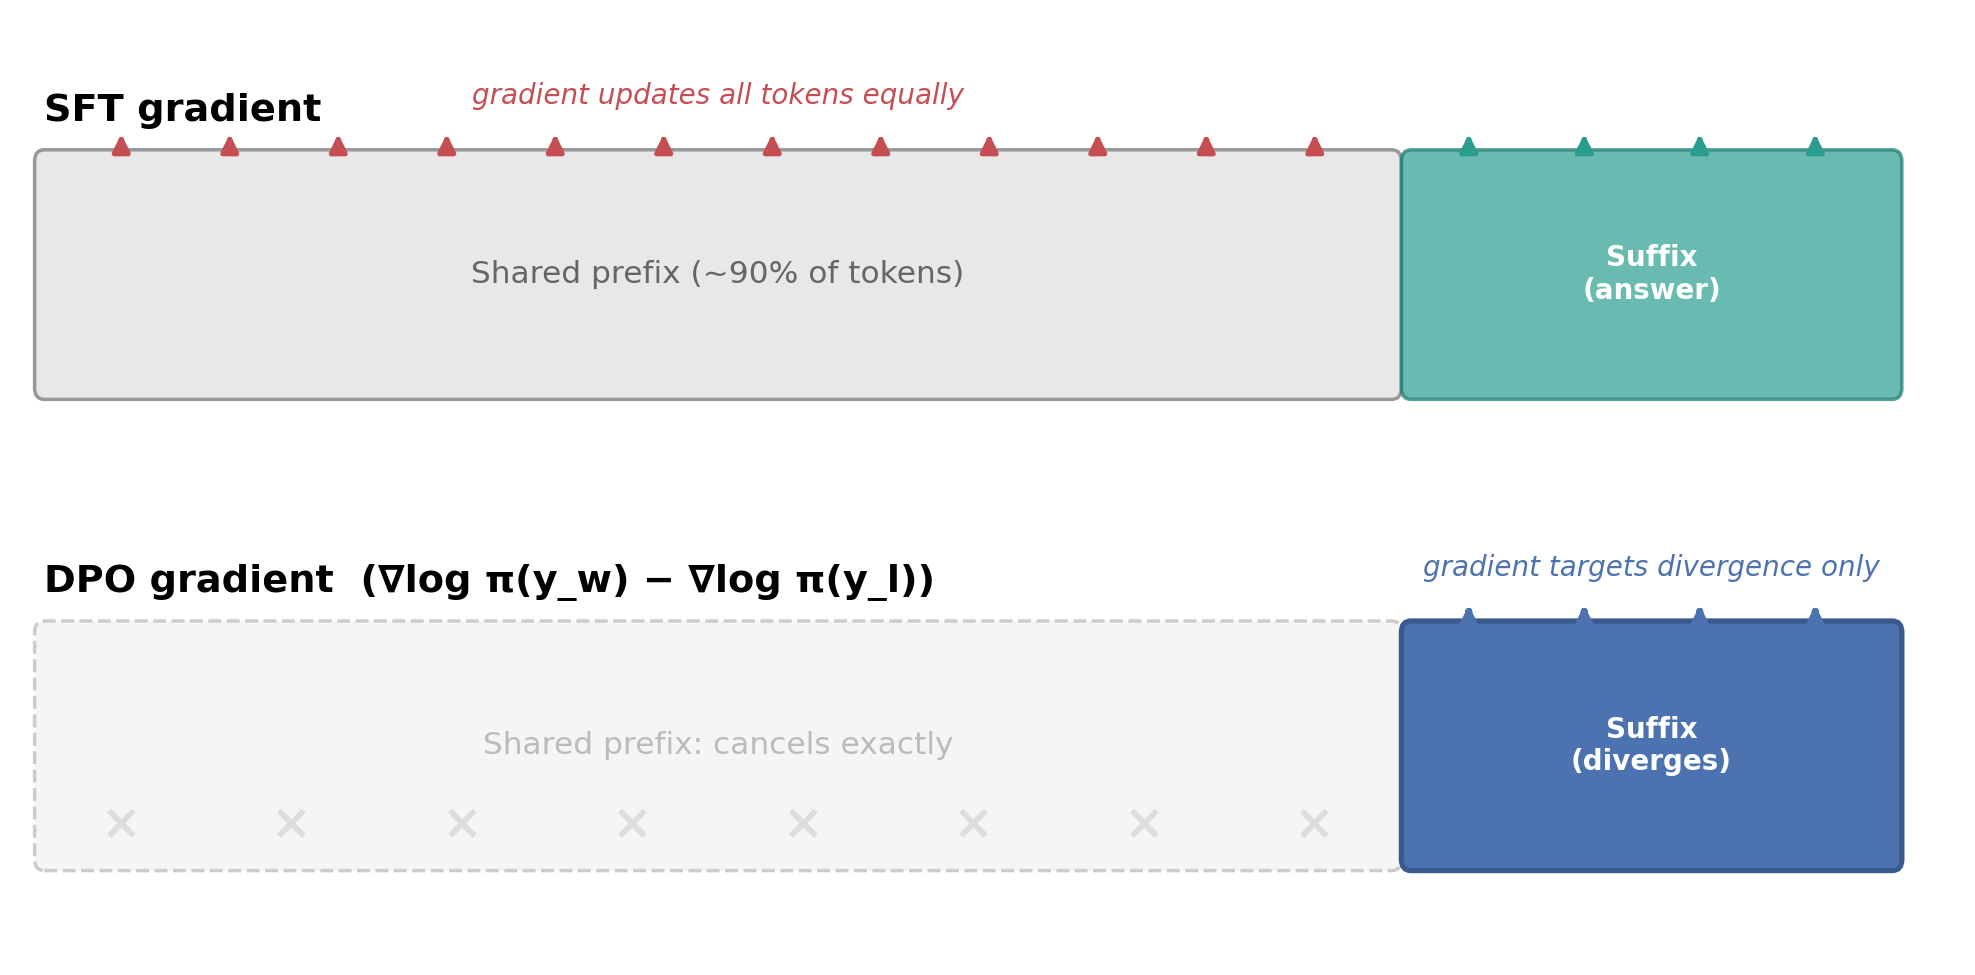
\includegraphics[width=\linewidth]{figures/gradient_cancellation.png}
    \caption{SFT updates all tokens including the shared prefix ($\sim$90\% of the sequence). DPO's contrastive gradient cancels the shared prefix, focusing updates on the divergent suffix.}
    \label{fig:gradient}
\end{figure}

\paragraph{Depth and correction yield.}
Correction yield varies with error-position depth: early positions ($<20\%$ depth) yield around 48\% correct corrections, dropping to around 29\% for late positions ($>80\%$ depth).
Early-divergence selection ($-0.8$pp) outperforming random ($-3.8$pp) in the correction experiment fits with this: earlier positions preserve more correct prefix, so the chosen response is higher quality despite the self-repair artifacts.

\paragraph{Reproducibility.}
Two separate evaluation runs of rollout DPO models produced different absolute base scores (76.0\% vs 74.2\%) but identical directional patterns---all rollout conditions above base in both runs.
Per-run variance of ${\sim}1.8$pp likely reflects vLLM non-determinism and LoRA merge differences.
The paired test controls for this by comparing outcomes on the same 500 problems within each run.

%--------------------------------------------------
\section{Conclusion}
\label{sec:conclusion}
%--------------------------------------------------

Correction-based DPO hurt in 3/3 conditions, rollout-based DPO helped in 5/5, and a matched replication brought the overall count to 10/11 ($p = 0.012$ by sign test, though conditions are not independent and baselines differ across experiments).
We went into this expecting corrections to fare better under DPO than under SFT, since DPO does not directly imitate the chosen text.
That turned out to be wrong---the correction data degraded performance either way.
An ablation (\S\ref{sec:analysis}) narrows the cause to the failed-reasoning prefix in correction pairs: removing the self-repair rhetoric alone does not help, but stripping the entire failed prefix recovers performance to baseline.

The biggest gap in this work is that the correction and rollout experiments started from different checkpoints with different hyperparameters.
The matched replication covers the correction side, but we still lack a rollout run from that same checkpoint, which means we cannot fully separate the data-source effect from training configuration.
We also tested only one model (Qwen3-8B), one benchmark (MATH-500), one seed per condition, and 150--228 pairs; no individual comparison survives Benjamini-Hochberg correction.

If we had more compute, the first thing we would run is the fully matched version: correction and rollout DPO from the same checkpoint, same $\beta$, same learning rate.
The ablation results raise an interesting possibility: if corrections are generated as standalone responses rather than continuations of failed reasoning, they might work as well as rollout pairs.
We did not have the compute to test this at scale.
Whether rollout-based gains hold at 1K--10K pairs or transfer to other model families is an open question we did not get to test.


%--------------------------------------------------
\appendix
%--------------------------------------------------

\section{Research Trajectory}
\label{app:trajectory}

The final design emerged from several earlier directions that did not produce usable results at the 7B--8B scale we operated at; some of these might work at larger scale or with more compute.

\paragraph{Phase A: Scaffold co-evolution.}
Inspired by Dynamic Cheatsheet~\cite{suzgun2025dc}, we tested whether a self-curating strategy scaffold could co-evolve with GRPO training to preserve reasoning diversity.
We used a kill-test: train with the scaffold, evaluate without it.
At 7B scale, removing the scaffold collapsed performance from 0.363 to 0.079 pass@1 (Table~\ref{tab:scaffold}).
At this scale, the model learned to depend on the scaffold rather than absorb it, though larger models with stronger in-context learning might behave differently.

\begin{table}[h]
    \centering
    \caption{Scaffold kill-test (Phase A). ``Removed'' = scaffold-trained model evaluated without scaffold.}
    \vspace{0.5em}
    \begin{tabular}{llccc}
        \toprule
        Scale & Condition & pass@1 & pass@8 & Oracle Gap \\
        \midrule
        3B & RL-only & 0.513 & 0.900 & 0.387 \\
        3B & RL + scaffold & 0.487 & 0.867 & 0.380 \\
        3B & Scaffold removed & 0.266 & 0.766 & 0.500 \\
        7B & RL-only & 0.553 & 0.940 & 0.387 \\
        7B & RL + scaffold & 0.363 & 0.700 & 0.337 \\
        7B & Scaffold removed & 0.079 & 0.433 & 0.354 \\
        \bottomrule
    \end{tabular}
    \label{tab:scaffold}
\end{table}

\paragraph{Phase B: Token-level fork signals.}
Wang et al.~\cite{wang2025beyond} identified ``fork tokens''---positions where correct and incorrect reasoning paths diverge---as driving RLVR learning.
We tested whether token entropy could identify these positions, but it produced a 42\% false-positive rate and 84\% of flagged tokens had zero outcome variance.
Token entropy measures next-token uncertainty, not whether the branch actually leads to a different answer; a richer signal (e.g., outcome variance across rollouts) might work but was outside our compute budget.

\paragraph{Phase C: Fork detection via hidden states.}
We tested five methods for single-pass fork detection (Table~\ref{tab:detection_app}).
None exceeded a position-only baseline (AUROC = 0.901).
The best probe (AUROC = 0.802) was picking up on the fact that forks tend to occur at certain depths, not on what makes a position a fork; with more data or larger models the hidden-state signal might become separable, but we could not demonstrate it here.

\begin{table}[h]
    \centering
    \caption{Five single-pass fork detection methods (Phase C). None exceeds a position-only baseline.}
    \vspace{0.5em}
    \begin{tabular}{llcc}
        \toprule
        Method & Signal & AUROC & Status \\
        \midrule
        Token entropy & Next-token $H$ & 0.58 (42\% FPR) & Failed \\
        Attention divergence & Per-head JSD & 0.480 & Failed \\
        Fork probe v1 & Hidden state classifier & 0.551 & Failed \\
        Fork probe v2 & Probe + position control & $0.802^\dagger$ & Failed \\
        Activation change & Norm change & 0.480 & Failed \\
        \bottomrule
    \end{tabular}
    \label{tab:detection_app}
    \vspace{0.3em}
    {\small $^\dagger$Position-only baseline: AUROC $= 0.901 > 0.802$.}
\end{table}

\paragraph{Phase D: DEEP-GRPO error-position pipeline.}
Since single-pass detection did not work at this scale, we moved to rollout-based identification using DEEP-GRPO~\cite{deepgrpo2026}.
The pipeline successfully identified error positions and generated corrections, but training on those corrections degraded performance (see below).

\paragraph{Phase E: From corrections to rollouts.}
SFT on correction data hurt performance (Appendix~\ref{app:sft}), and DPO on the same correction data also hurt (Table~\ref{tab:correction}).
Removing correction-derived text and pairing natural rollouts reversed the effect (Table~\ref{tab:rollout}), which pointed to the data source as the key variable rather than the training algorithm.

\section{Pipeline Analysis}
\label{app:pipeline}

\paragraph{Error-position identification.}
We use DEEP-GRPO's~\cite{deepgrpo2026} depth-biased position selection on the 141 mixed-outcome problems.
The logistic recoverability estimator $P_\phi$ is fit online: uniform sampling for the first 10 problems, refit every 10 problems thereafter.
Segmentation uses \texttt{\textbackslash n\textbackslash n} (paragraph) boundaries.

\paragraph{Correction yield.}
Starting over from position 0 (root resample) corrects 58.2\% of traces; correcting mid-trajectory at DEEP-GRPO positions corrects only 33.6\% (Table~\ref{tab:yield}).
The depth bias ($\gamma = 2$) selects late positions (mean depth 0.709) where the model has less room to recover.

\begin{table}[h]
    \centering
    \caption{Correction yield by method.}
    \vspace{0.5em}
    \begin{tabular}{lccc}
        \toprule
        Method & Yield & $n_{\text{correct}} / n_{\text{total}}$ & Mean Depth \\
        \midrule
        Root resample (Best-of-$N$) & 58.2\% & 4,876 / 8,384 & 0.0 \\
        First divergence (oracle) & 48.2\% & 1,779 / 3,688 & varies \\
        Random position & 37.3\% & 1,376 / 3,688 & $\sim$0.50 \\
        DEEP-GRPO ($\gamma = 2$) & 33.6\% & 1,323 / 3,936 & 0.709 \\
        \bottomrule
    \end{tabular}
    \label{tab:yield}
\end{table}

\paragraph{Yield by difficulty and subject.}
Level 1 problems have the lowest correction yield (21.0\%) because most are already solved by all 8 rollouts and only enter the mixed-outcome set when a single rollout fails---leaving little room for correction to improve on.
By subject, algebra corrections succeed most often (63.2\%) and geometry least (32.0\%), as shown in Table~\ref{tab:level_subject}.

\begin{table}[h]
    \centering
    \caption{Correction yield by difficulty level (left) and subject (right).}
    \vspace{0.5em}
    \begin{minipage}{0.45\textwidth}
        \centering
        \begin{tabular}{lcc}
            \toprule
            Level & Yield & $n$ \\
            \midrule
            1 & 21.0\% & 176 \\
            2 & 55.0\% & 400 \\
            3 & 63.0\% & 648 \\
            4 & 55.7\% & 776 \\
            5 & 42.5\% & 1,936 \\
            \bottomrule
        \end{tabular}
    \end{minipage}
    \hfill
    \begin{minipage}{0.50\textwidth}
        \centering
        \begin{tabular}{lcc}
            \toprule
            Subject & Yield & $n$ \\
            \midrule
            Algebra & 63.2\% & 280 \\
            Count.\ \& Prob.\ & 41.6\% & 392 \\
            Geometry & 32.0\% & 440 \\
            Intermed.\ Algebra & 43.6\% & 1,336 \\
            Number Theory & 67.3\% & 392 \\
            Prealgebra & 50.4\% & 520 \\
            Precalculus & 57.3\% & 576 \\
            \bottomrule
        \end{tabular}
    \end{minipage}
    \label{tab:level_subject}
\end{table}

\section{SFT Ablation}
\label{app:sft}

We first tried SFT on correction data before switching to DPO.
Adding 116 correction traces to 465 clean traces (Model B in Table~\ref{tab:sft}) lost 6.5pp on recovery rate and 5.0pp on pass@1 relative to clean-only SFT (Model A).
A volume control with 2000 oversampled clean traces (Model C) matched the untrained base, suggesting the clean traces themselves had limited value beyond establishing the SFT checkpoint.

\begin{table}[h]
    \centering
    \caption{SFT ablation on correction data. QLoRA $r{=}64$, 5 epochs.}
    \vspace{0.5em}
    \begin{tabular}{llcc}
        \toprule
        Model & Training Data & Recovery & Pass@1 \\
        \midrule
        Base & None (Qwen3-8B) & 0.575 & 0.400 \\
        A & Clean traces (465) & 0.591 & 0.550 \\
        B & Clean + corrections (581) & 0.526 & 0.500 \\
        C & Volume control (2000) & 0.561 & 0.400 \\
        \bottomrule
    \end{tabular}
    \label{tab:sft}
\end{table}

After this, we tried DPO on the same correction data, reasoning that a contrastive objective would not directly imitate the correction text and might avoid copying the out-of-distribution artifacts.
As reported in Table~\ref{tab:correction}, the correction-based DPO pairs also hurt, though less severely than SFT.

\section{MATH-500 Rollout Statistics}
\label{app:stats}

\begin{table}[h]
    \centering
    \caption{Rollout statistics ($N = 8$ per problem, Qwen3-8B).}
    \vspace{0.5em}
    \begin{tabular}{lc}
        \toprule
        Metric & Value \\
        \midrule
        Total problems & 500 \\
        Mean accuracy & 72.9\% \\
        Mixed-outcome ($1 \leq \text{correct} \leq 7$) & 141 (28.2\%) \\
        All correct (8/8) & 311 (62.2\%) \\
        All incorrect (0/8) & 48 (9.6\%) \\
        Total corrections generated & 3,936 \\
        Unique error positions & 492 \\
        Correct corrections & 1,323 (33.6\%) \\
        Problems with $\geq 1$ correct correction & 125/141 (88.7\%) \\
        Mean pairwise diversity & $0.617 \pm 0.110$ \\
        \bottomrule
    \end{tabular}
    \label{tab:rollout_stats}
\end{table}

\bibliographystyle{unsrt}
\bibliography{references}

\end{document}
